\section{Model and Problem}\label{sec:model}

\subsection{The Fleet and the Question}
A fleet of $N$ vessels tows one payload, each through one cable loaded to the pretension $T_0$ in steady tow. The cables are unilateral Kelvin--Voigt lines, with tension $[k e_i+c\dot e_i]_+$ for elongation $e_i>0$ and none otherwise \cite{hall2015validation}; the clamp keeps the damper from pushing in compression just before separation \cite{hunt1975coefficient}. When cable $j$ re-engages with closing speed $V=\dot e_j(0^+)>0$, its tension reaches $\Tp$ and returns to zero after a finite contact. We call this a \emph{snap} (Fig.~\ref{fig:fleetsnap}) and define the transmission to neighbor $i$ by
\begin{equation}\label{eq:rho}
  \rho_{ij}=\frac{\max_t\Delta T_i(t)}{\Tp},\qquad \Tp=\max_t T_j(t),
\end{equation}
where $\Delta T_i$ is the drop relative to the counterfactual tension without the snap. Section~\ref{subsec:magnitude} realizes the counterfactual numerically.

\begin{figure}[t]
  \centering
  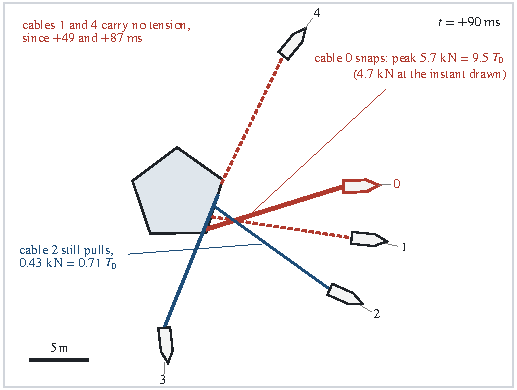
\includegraphics[width=\columnwidth]{fig_fleet_snap}
  \caption{A selected, atypical snap on the testbed ($T_0=0.6$\,kN), $90$\,ms after cable~0 re-engages; taut cables solid (width growing with tension), slack cables dashed. Cable~0 peaks at $9.51T_0$, far above the scored range $[T_0,4T_0]$, at $58$\,ms. Cable~1, already near slack ($0.66T_0$), reaches zero at $49$\,ms; cables 4 and 3 follow at $87$ and $206$\,ms; cable~2 stays taut for one engagement period.}
  \label{fig:fleetsnap}
\end{figure}

\subsection{Collinear Reduction}
Section~\ref{sec:test} measures the cost of the following idealization on a planar fleet.
\begin{assumption}\label{ass:collinear}
The cables are parallel and attached so a snap does not rotate the payload; all have stiffness $k$ and damping $c$, the vessels share mass $m_A$ and drag $c_A$, and the payload has mass $m_L$ and drag $c_L$. During one snap, thrust and weather forces are constant, so they cancel in the perturbation about the steady tow, and the $N-1$ neighbors begin from a common taut state of tension $\Tn>0$.
\end{assumption}
Let $x$, $y_j$, and $y$ be payload, parent-vessel, and neighbor-vessel displacements from steady tow; by symmetry and uniqueness the neighbors move together.
\begin{assumption}\label{ass:wellposed}
Solutions cross the switching surface $e_j=0$ transversally, so the hybrid solution is unique.
\end{assumption}
While the neighbors remain taut,
\begin{equation}\label{eq:model}
\begin{aligned}
  m_L\ddot x &= f+(N-1)\delta T-c_L\dot x,\\
  m_A\ddot y &= -\delta T-c_A\dot y,\\
  m_A\ddot y_j &= -f-c_A\dot y_j,
\end{aligned}
\end{equation}
with $\delta T=k(y-x)+c(\dot y-\dot x)$, $f=[ke_j+c\dot e_j]_+$ for $e_j=y_j-x>0$ and $f=0$ otherwise, and zero initial state except $\dot y_j(0)=V$. Hence $\Delta T=-\delta T$ and $\rho=\max\Delta T/\max f$ over the first contact and its response; a later contact of cable $j$ is a new snap. For prescribed $f$, \eqref{eq:model} is linear, so the snap contribution is a superposed perturbation; the nonlinear planar testbed instead uses paired re-integrations with and without the snapping-cable force, a counterfactual rather than a superposition.

\subsection{The Impulsive Estimate}
Replace the contact by an impulse $J=\int f\,dt$, hold the neighbor vessels ($y\equiv0$), and ignore dissipation. The payload leaves with velocity $J/m_L$ and oscillates at $\omega_L=\sqrt{(N-1)k/m_L}$, giving $\max\Delta T=kJ/(m_L\omega_L)$. For an isolated half-sine contact $f=\Tp\sin\omega_e t$ on $[0,\pi/\omega_e]$, with $\omega_e=\sqrt{k(1/m_A+1/m_L)}$, $J=2\Tp/\omega_e$ and
\begin{equation}\label{eq:imp}
  \rhoimp=\frac{2k}{m_L\omega_L\omega_e}.
\end{equation}
Equivalently, $\rhoimp=(2k/(\omega_L\omega_e))\,[W^\top M_L^{-1}W]_{ij}$, where $W$ has the cable wrenches $(d_i,r_i\times d_i)$ as columns, with unit chord $d_i$ and attachment arm $r_i$, and $M_L=\operatorname{diag}(m_L,m_L,I_L)$; under Assumption~\ref{ass:collinear} the lever arms vanish and the off-diagonal entry is $1/m_L$.
At $N=5$ and $m_A/m_L=0.24$, \eqref{eq:imp} gives $\rhoimp=0.440$, so a neighbor at $T_0$ would unload near $2.3T_0$. It is the direct impact construction, not a published law; we use it as the baseline and remove its finite-contact and held-end assumptions below.
